\documentclass{acm_proc_article-sp}
\usepackage{hyperref}


\makeatletter

\def\somemagiccommand#1{%
\let\tc@w\@empty
\protected@edef\tmp{\noexpand\tc@a#1\relax}\expandafter\tc@uc@\tmp}

\def\tc@a{\futurelet\tmp\tc@aa}

\def\tc@aa{%
\ifcat a\noexpand\tmp\expandafter\tc@ab
\else\expandafter\tc@ac\fi}

\def\tc@ab#1{\edef\tc@w{\tc@w#1}\tc@a}

\def\tc@ac{%
\csname tc@@\tc@w\endcsname\expandafter\tc@uc\tc@w
\let\tc@w\@empty
\ifx\tmp\@sptoken\let\next\tc@sp
\else\ifx\tmp\relax\let\next\relax
\else\let\next\tc@nxt
\fi\fi\next}

\def\tc@sp#1{ \tc@a#1}
\def\tc@nxt#1{#1\tc@a}

\def\tc@uc#1{\uppercase{#1}}
\def\tc@uc@#1#2{\uppercase{#1#2}}

\let\tc@@the\@gobbletwo
\let\tc@@and\@gobbletwo

\makeatother


\begin{document}
\title{Using Bayesian Networks to Predict March Madness Brackets and Results}
\numberofauthors{2}
\author{
\alignauthor
Kenneth Stewart II\\
       \affaddr{Rochester Institute of Technology}\\
       \email{kis7255@g.rit.edu}
\alignauthor
Marko F. Galesic\\
       \affaddr{Rochester Institute of Technology}\\
       \email{mfg1071@g.rit.edu}
}
\maketitle
\begin{abstract}
Generally, we will use standard statistical basketball indices for team performance to create a 
model that can predict whether a team will win March Madness given the season statistics and 
tournament seeds. We intend to develop an algorithm to parse the initial dataset and derive features 
from the data to create a table of statistical indices for each team a the given season. The seasons 
are then aggregated together to come up with an over performance history of each team. The 
statistical indices will then be used as input to a Baysian Network to create probabilities for the
winner of each game in the tournament until a tournament winner is chosen.
\end{abstract}
\section{Bayesian Networks Literature Review}
Bayesian (Belief) Networks is a probabilistic graphical model used to model knowledge about an 
uncertain domain. Each graph node represents a random variable and each edge between nodes 
represents the probabilistic dependencies among the corresponding nodes\cite{heckerman}.
The edges are often estimated using various statistical and numerical methods such as observations 
made by the Chain Rule (discussed later).\cite{wagner, tan} 
Bayesian Networks are structured as directed acyclic graphs (DAG) which enables an intuitive, rigorous model that effectively represents and facilitates the computation of the joint probability distribution over a set of random variables\cite{heckerman}. These graphs are structured as two sets, one for nodes and one for directed edges. An edge from node 'i' to node 'j' means the value taken by node 'j' depends on the value of node 'i', meaning node 'i' influences node 'j', making node 'i' one of the parents of node 'j' and node 'j' a child of node 'i'\cite{heckerman}. Nodes that represent variables are evidence nodes, otherwise they are latent or hidden nodes. We've reviewed literature that goes through various techniques available in WEKA, the data mining and learning tool.\cite{weka}
\newpage
\section{Data Preprocessing}
\subsection{Data Cleaning}
Since the data primarily consists of continuous and the ranges of data are given, we can use 
clustering techniques to aid in a more efficient process to validate the data. Google refine will be 
used to handle this task. The source documented three (3) records that were added to create a 
complete the dataset that was representative of all the current team eligible for the tournament. We 
chose to remove these entries from the set as they may compromise our model as the data for the 
records are sparse.
\subsection{Stratified Sampling}
The dataset is not large (several megabytes), but we can still split on seasons to make processing 
the data faster. Instead of processing each game of every season. A subset of the first 'n' games 
for each team for each season will be used. This effectively reduces the data the data by a constant 
factor each time 'n' decreases by a constant factor. This also effectively helps reduced the time 
for pre-processing while still accurately representing the model as long a significant amount of 
games are used.
\subsection{Aggregation \textbackslash Feature Creation}
We plan to use the following measures and indices to predict teams' chances of winning the NCAA 
Division I championship: Rating Percentage Index (RPI), Average Margin of Victory, Pythagorean 
Expectation, and Close Won Games. Each index provides different descriptive features of a team. 
These features are then used to construct the Bayesian Network to model the joint probability 
distribution of the variables. These features will be calculated per team over all seasons giving us 
a total of 356 records. The records then become input to a Bayesian Network to generate 
probabilities to calculate the winner of each game starting from the first round all the way to the 
championship game to determine a winner. Following is the rationale behind each metric.
\subsubsection{Rating Percentage Index (RPI)}
While we've read that RPI is not a good indicator of team performance since it does not include a 
team's defensive fitness\cite{mozell}, several contestants for the March Machine Learning Madness 
competition have mentioned that they are using RPI in their algorithms.\cite{sonas, crowson, 
covalytics} It is a common indicator of team performance.
\subsubsection{Average Margin of Victory}
Average Margin of Victory will give us information on how much, on average, a team performed better 
than another team. It is a relative measure of team fitness or "goodness", and so we include it as 
one of our features to have a relative metric. It also has an interesting relationship with 
pythagorean expectation (Fig. 1).
\begin{figure}
\centering
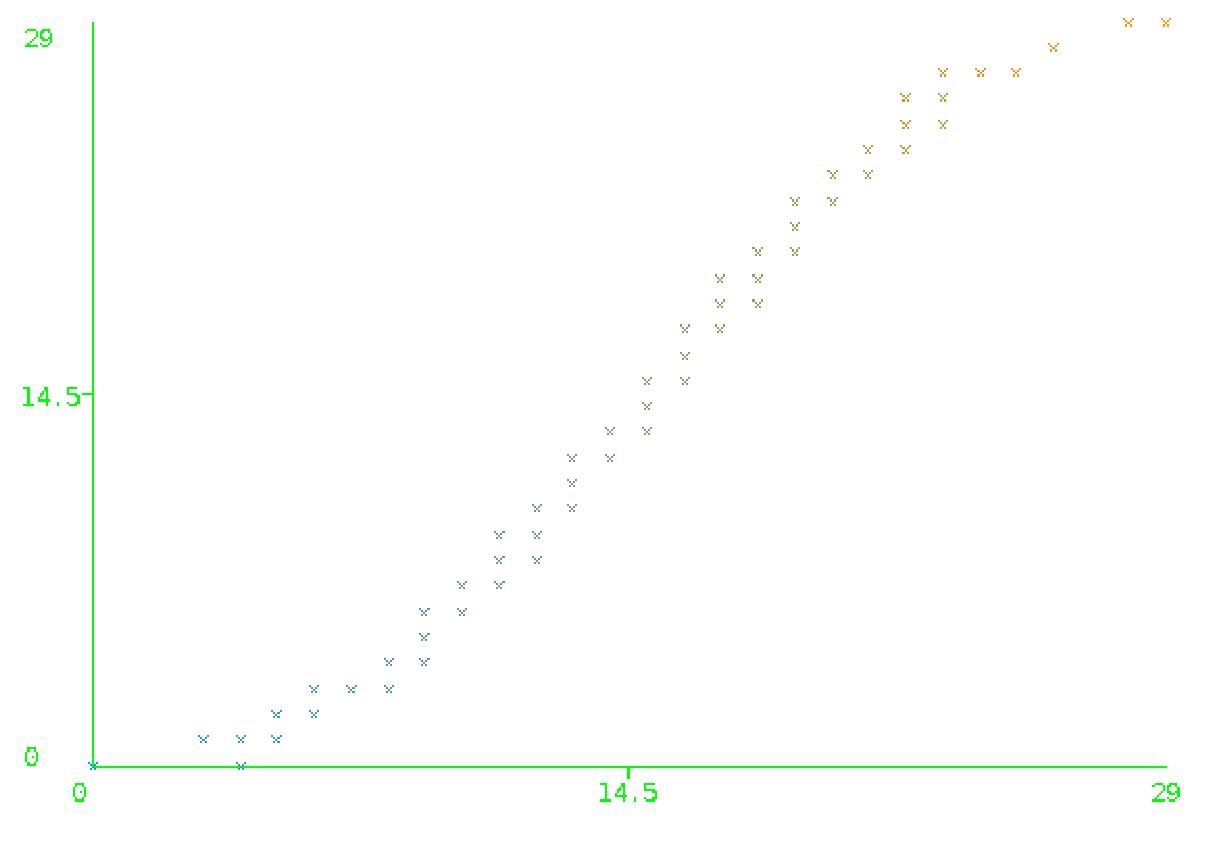
\epsfig{file=avg_pyth.eps, height=2in, width=2in}
\caption{A scatterplot of Average Margin of Victory(X) vs. Pythagorean Expectation(Y)}
\end{figure}
\subsubsection{Pythagorean Expectation}
This index was developed by Daryl Morey, a sports executive, who had much success in turning around 
a losing team into a successful team.\cite{feschuk} Pythagorean expectation seems to have its roots 
in the Pythagorean theorem and may be rooted better theoretically than RPI. RPI and Pythagorean 
Expectation are similar and are roughly correlated.
\subsubsection{Close Won Games}
This metric does not seem to be correlated with either RPI, Pythagorean expectation, or Average 
Margin of Victory, meaning that we'd get more information from close won games than from just RPI or 
Pythagorean expectation. The Fig. 2 and 3 show for Close Won Games versus RPI or Pythagorean 
Expectation show there is little correlation between these attributes.
\begin{figure}
\centering
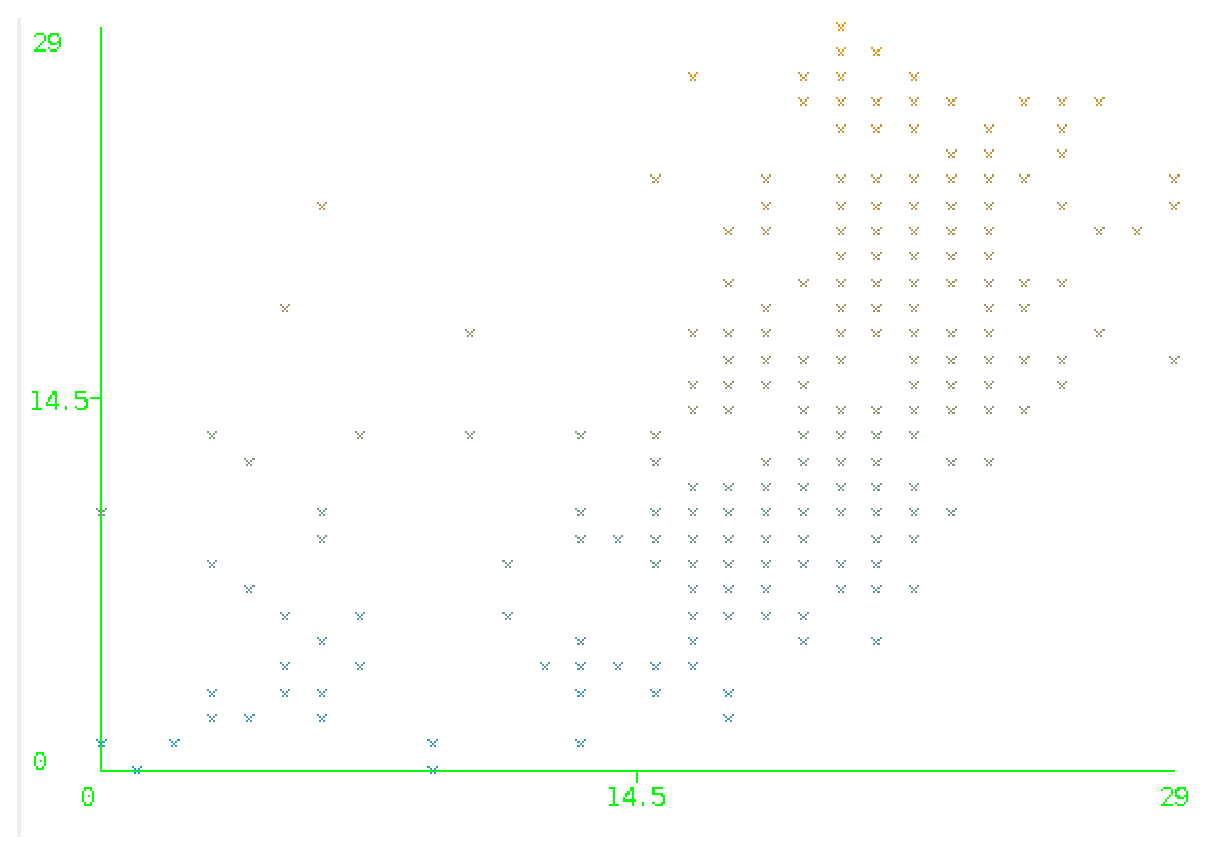
\epsfig{file=cwg_pyth.eps, height=2in, width=2in}
\caption{A scatterplot of Close Won Games(X) vs. Pythagorean Expectation(Y)}
\end{figure}
\begin{figure}
\centering
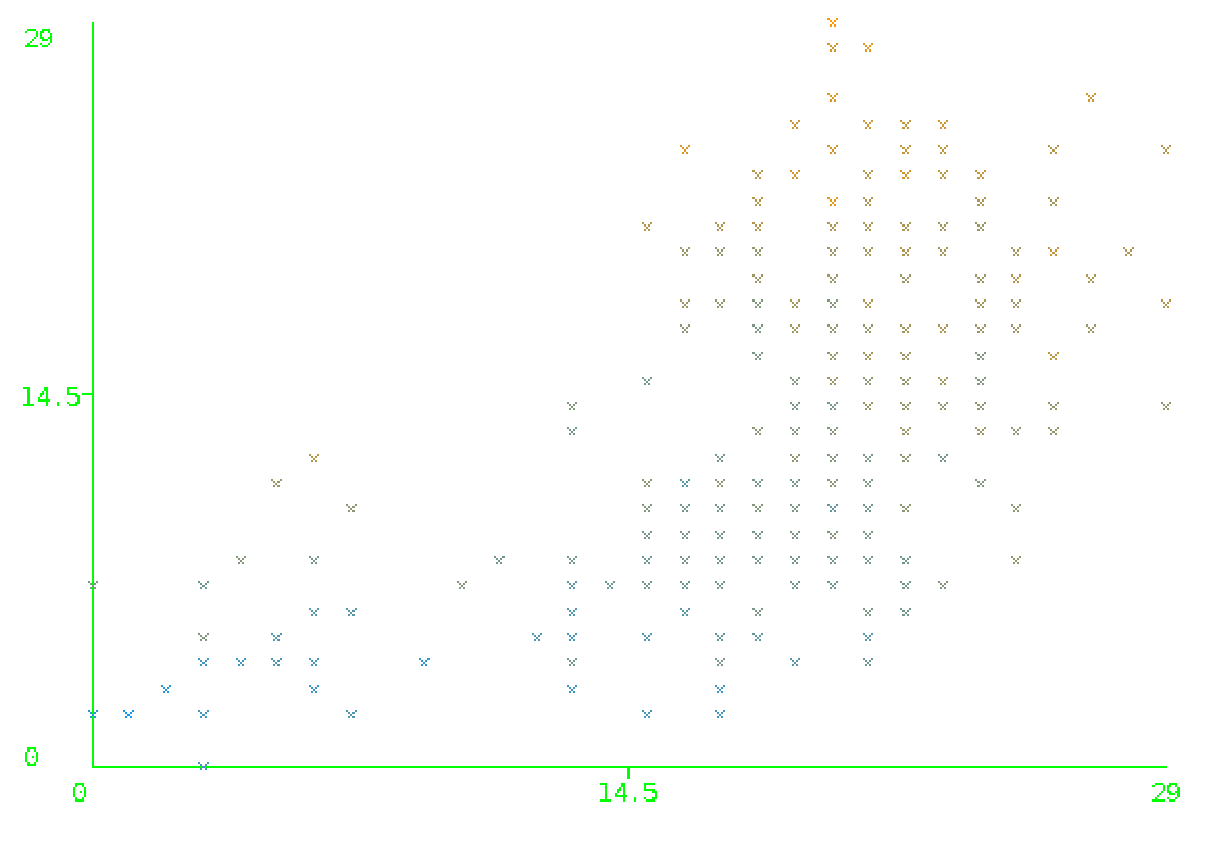
\epsfig{file=cwg_rpi.eps, height=2in, width=2in}
\caption{A scatterplot of Close Won Games(X) vs. Pythagorean Expectation(Y)}
\end{figure}
The graph of Close Won Games versus Average Margin of Victory is similar. This should not be a 
surprise since Average Margin of Victory has a correlation with the Pythagorean Expectation.
\section{Structure of Training \textbackslash Test Sets}
Out of the eighteen (18) seasons given in the dataset. 11 of the seasons will be used for training 
data, the remaining 7 will be used for the test data (a 60/40 split). Our model will represent the 
regular season and the Division 1 Championship. Since teams come and go, it would be unwise to make 
specific models off teams. A larger practical concern if we modeled individual teams would be that 
we would end up having to train roughly 350 different models. On the other hand, we chose not to 
take into account schedule strength or the strength of a teams' conference as the NCAA ranking 
system does. This choice was made to reduce complexity.

In order to get variability in the dataset stratified sampling will be used to sample the 18 seasons 
worth of data we are given in the following way to create the training and test sets. First, given 
the seasons are in chronological order, the season are separated into three (3) groups that spans 
six (6) seasons each. This is done to help prevent bias in the model as the teams of today play 
differently then teams of yesterday due to enhancements in rules, medicine, training, and strategy. 
These variations must be captured  during the training process or the classification of a winner may 
be incorrectly chosen based on data that no longer accurately represents the model. Lastly, four (4) 
samples from two (2) groups will be selected and three (3) samples from the remaining group will be 
selected as training data (11 seasons total). The rest of the data will be used for testing.

The data will then be binned to discretize the continuous variables to better fit how our model 
(Bayesian Network) operates. Bayesian Networks generally operate on discrete variables. Continuous 
variables can be modelled, but must still be discretized.\cite{cobb} Discretization will let us 
create tables of local probability distributions for a particular node (representing a variable) 
given the node's parents. We plan on using a number of bins to represent the distribution of the 
data into well defined classes and possibly vary binning per continuous attribute to improve 
performance and perhaps avoid bias. Since most of the data has a normal distribution, equal width 
binning is the method of choice.
\newpage
\section{Bayesian Network}
\subsection{Constructing the Network}
Constructing a Bayesian Network is a multistep process with many variations depending on the 
application domain. We will be creating a predictive model and have focused our attention on 
algorithms that allow us to do so; however, the first step in the process is always to identify the 
variables of interest that the network is to model. We have outlined the variables (features) we are 
to use, statistical indices, in the previous sections.

The next step in the process is to create the actual structure of the network (the DAG). There are 
various ways to do this. One of the two methods in \cite{heckerman} outlined an algorithm that takes 
a set of variables (X = {x1, x2,..., xn}) in a particular order and computes the network based on 
the observations of the Chain Rule of Probability which says "PLACE THE EQUATION 17 from \cite
{heckerman} here". This is saying that the probability of a variable in the set X is equal to the 
product of each variable given all the variables that come before it. This identifies conditionally 
independent nodes (nodes with no parents) in the network as well as the connections between the 
conditionally dependent nodes. Thus, if a variable 'a' is conditionally dependent on a set of 
variables B then 'a' will have all variables in B as parents. This approach is the most 
straightforward; however, it has serious limitations. The ordering of variables is very sensitive 
and improper order can cause incorrect causal relationships to be formed which can lead to poor 
results.

The second approach is based on two observations: 1. People are able to readily assert causal 
relationships in the variables. 2. Causal relationships usually corresponds to assertions of 
conditional dependence \cite{heckerman}. Using these observations the person constructing the 
network can explicitly create nodes and connections. This usually preserves the observations from 
the Chain rule of Probability \cite{heckerman}.

The last step in the algorithm is to compute the local conditional probability distributions at each 
node in the graph. This is done by calculating, for each node, a single distribution for every 
combination of the configuration of the node's parents. The local conditional probability tables for 
each node will be calculated from data. This is accomplished by parsing the binned data, locating 
positives classes (wins), and determining the probability based on the number of positive 
observations divided by the number of observations. This is done for each combination of the binned 
attributes calculated after features have been extracted.
\subsection{Probabilistic Inference}
Probabilistic inference is the process of calculating a probability of interest from the model. 
There are two types of inference, approximate and exact. Exact inference is an NP-Hard problem. Due 
to this nature we chose to use approximate inference as it is less computationally expensive to 
compute. We are currently looking into algorithms that will allow efficient computation of an 
approximate value to used as the probability estimate. \cite{heckerman} has lead to additional 
resources to gain 
a better understanding of inference and the algorithms to compute probabilities of random variables.
\newpage
\section{Next Steps and Thoughts}
"Cinderella" and "Fatigue" Factors
We may weight each outcome with a "Cinderella" factor which would be a distribution we'd create 
based on low seed teams beating higher seed teams. This distribution could be put into either the 
table or as a scalar going in.
\begin{figure}
\centering
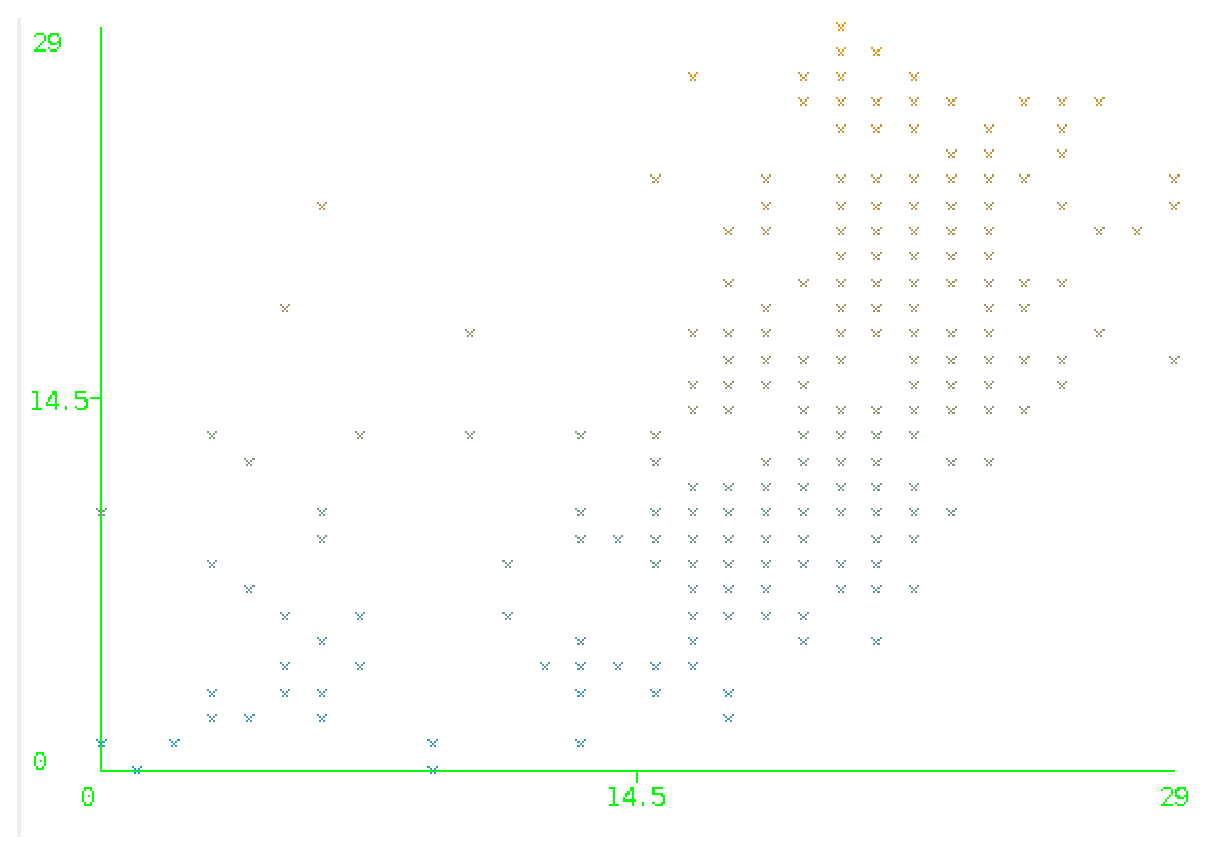
\epsfig{file=cwg_pyth.eps, height=2in, width=2in}
\caption{A scatterplot of Close Won Games(X) vs. Pythagorean Expectation(Y)}
\end{figure}
We may also use a function to represent how a given team would perform given the number of 
consecutive days said team has played. The function, we call it Fatigue, would scale a team’s 
probability of winning against any other team down the more consecutive games they have played. In 
March Madness, for example, the First Four are played almost a week in advance of the first round 32 
games, but then teams that have won in that first round would play another team within two days, 
whether or not the former are a high performing team or not. Fatigue would be dependent on a team’s 
baseline performance, a higher performing team would likely get fatigued slower than a lower 
performing team. A high seeded and low seeded team’s fatigue graph might look like Fig. 4.
\subsection{Probabilistic Inference Techniques}
One of our next goals is to really understand how to calculate probabilities from the Bayesian 
Network. We have encountered sources that lead to more descriptive explanations of probabilistic 
inference in Bayesian Networks. The next step is to review these sources and see what techniques fit 
our application domain well and make a decision of what to use.\cite{ruiz, ben}
\subsection{Learning Model}
Another short-term goal is to determine how the network is fine-tuned and the learning model is 
incorporated. Both the parameters and probabilities of a network can be fine-tuned \cite{heckerman}. 
We are working to determine how. 
\newpage
\bibliographystyle{ieeetr}
\bibliography{sigproc}
\end{document}
